\subsection{بخش ز}
این بخش به بررسی مانور هدف پرداخته شده است. همانطور از که نتایج مشخص است، مانور سناریو سوم سبب کاهش فاصله ازدست‌دهی شده است.

\begin{figure}[H]
	\centering
	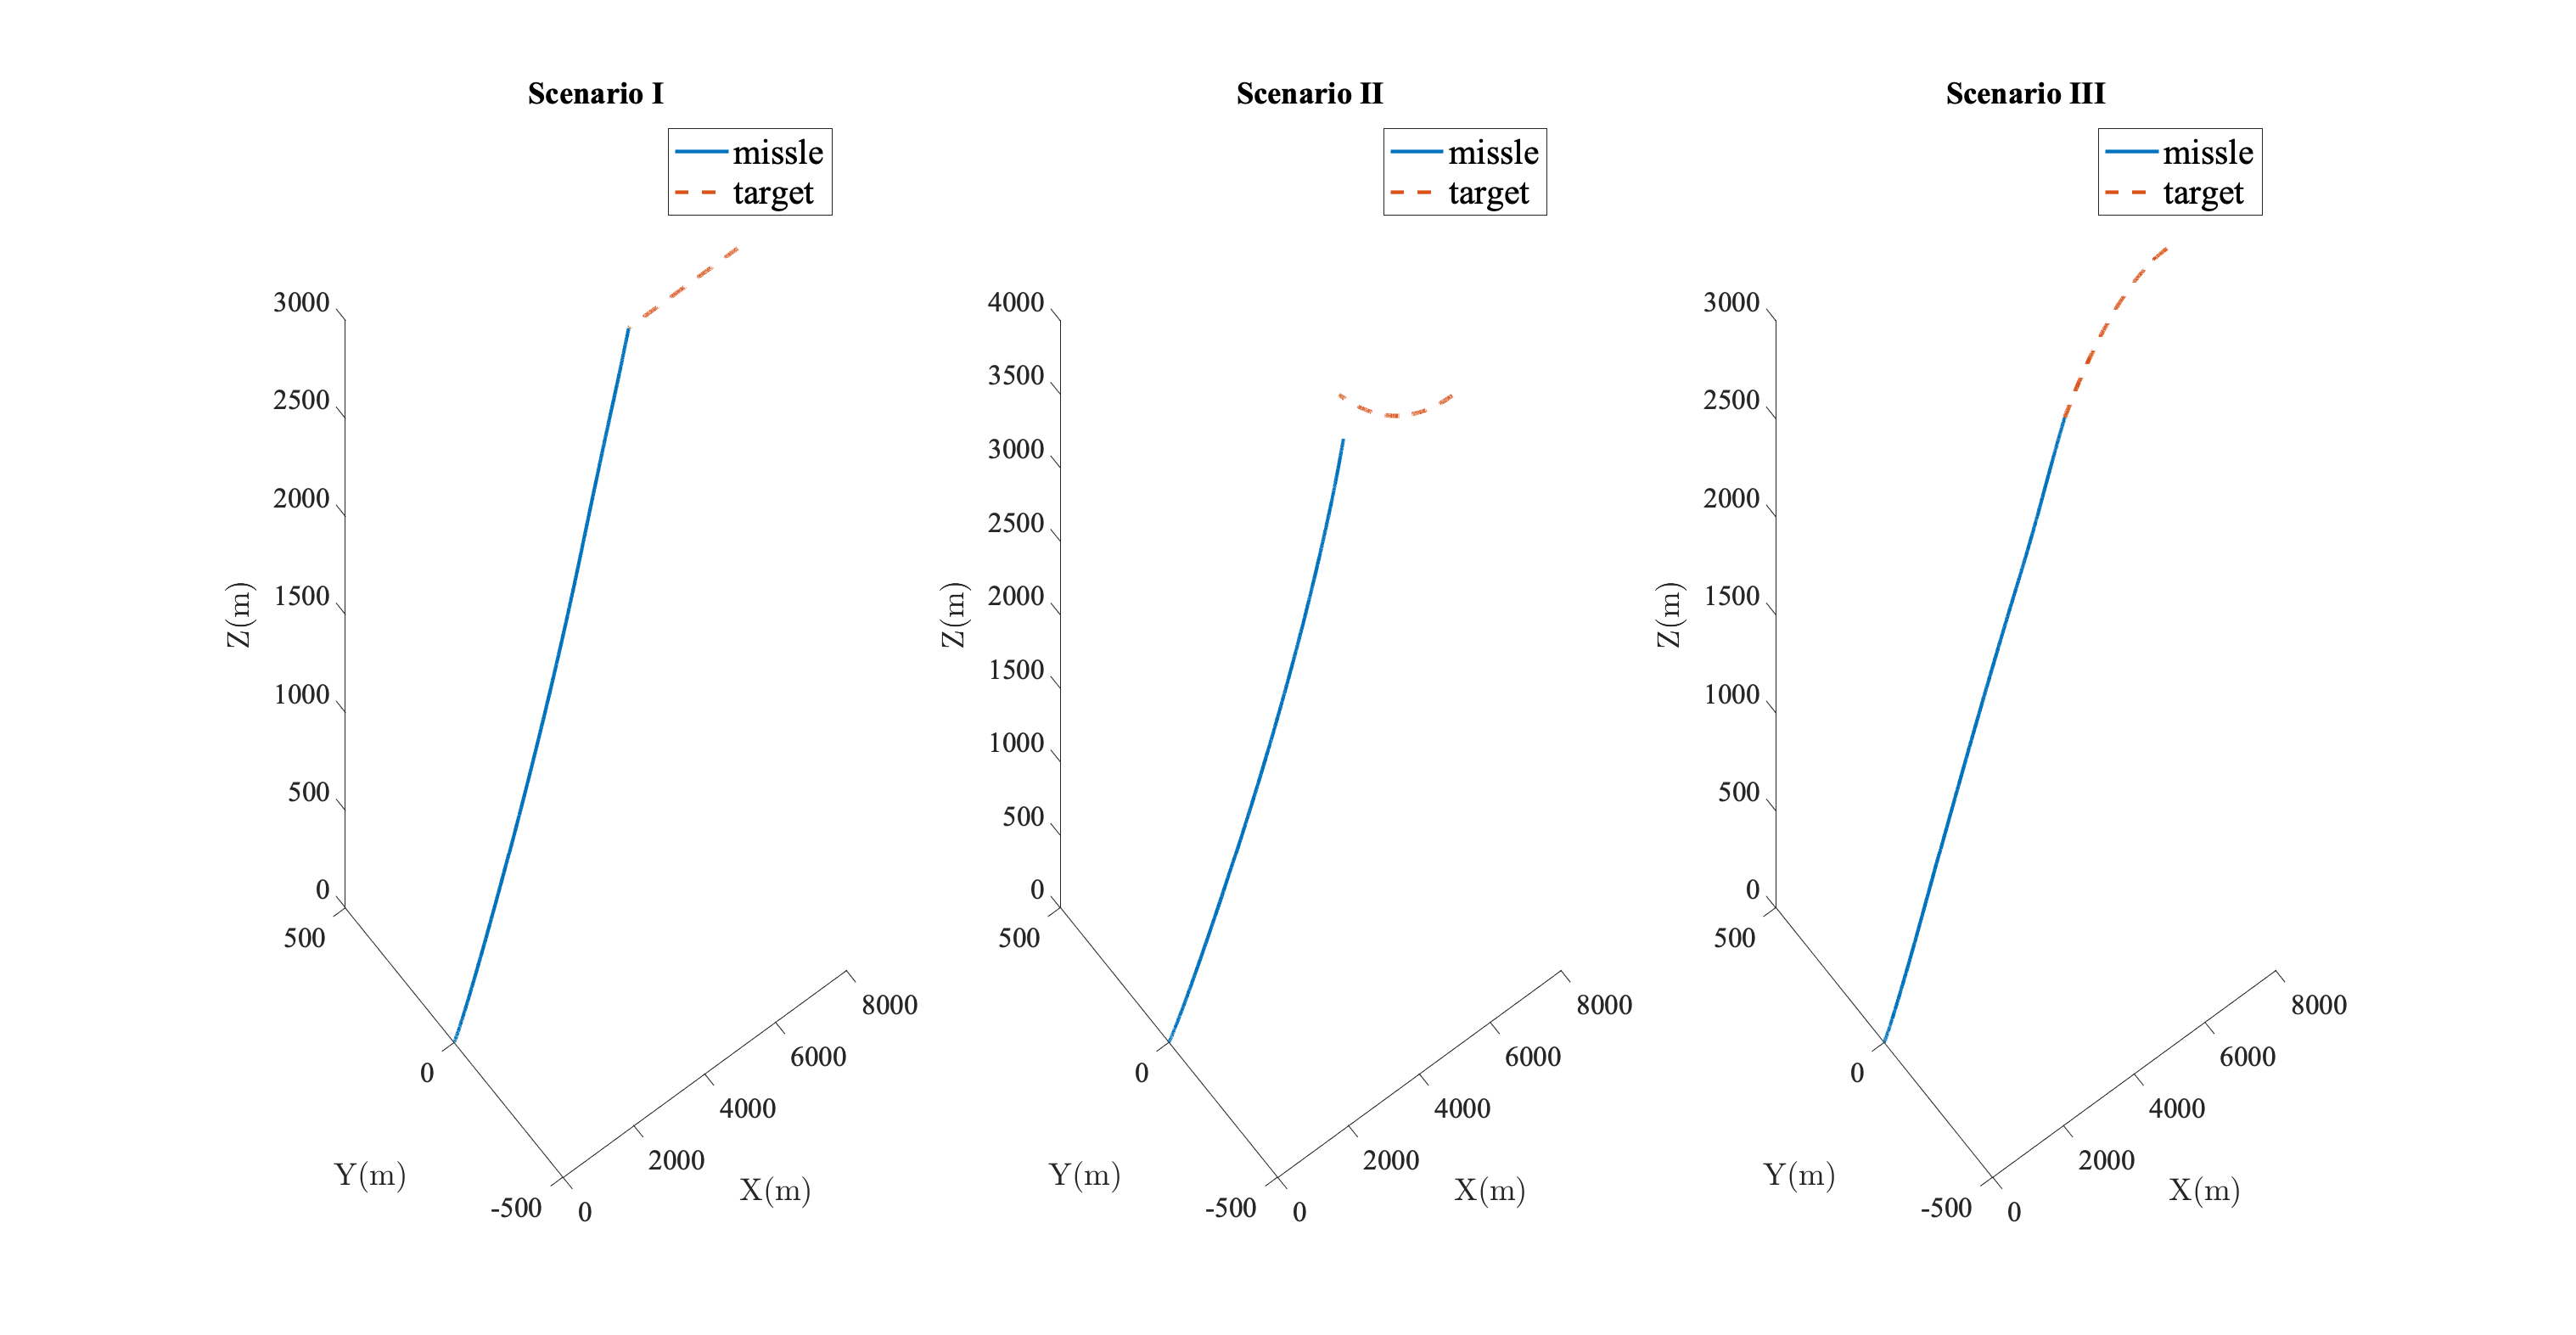
\includegraphics[width=\linewidth]{../Figure/m/3DoF_missle_vs_target_state_lead_angle_all_scenario}
	\caption{مقایسه موقعیت موشک و هدف به صورت سه بعدی در دو نمودار  در قانون هدایت فرمان به خط دید همراه با مانور هدف
	}
\end{figure}


\begin{figure}[H]
	\centering
	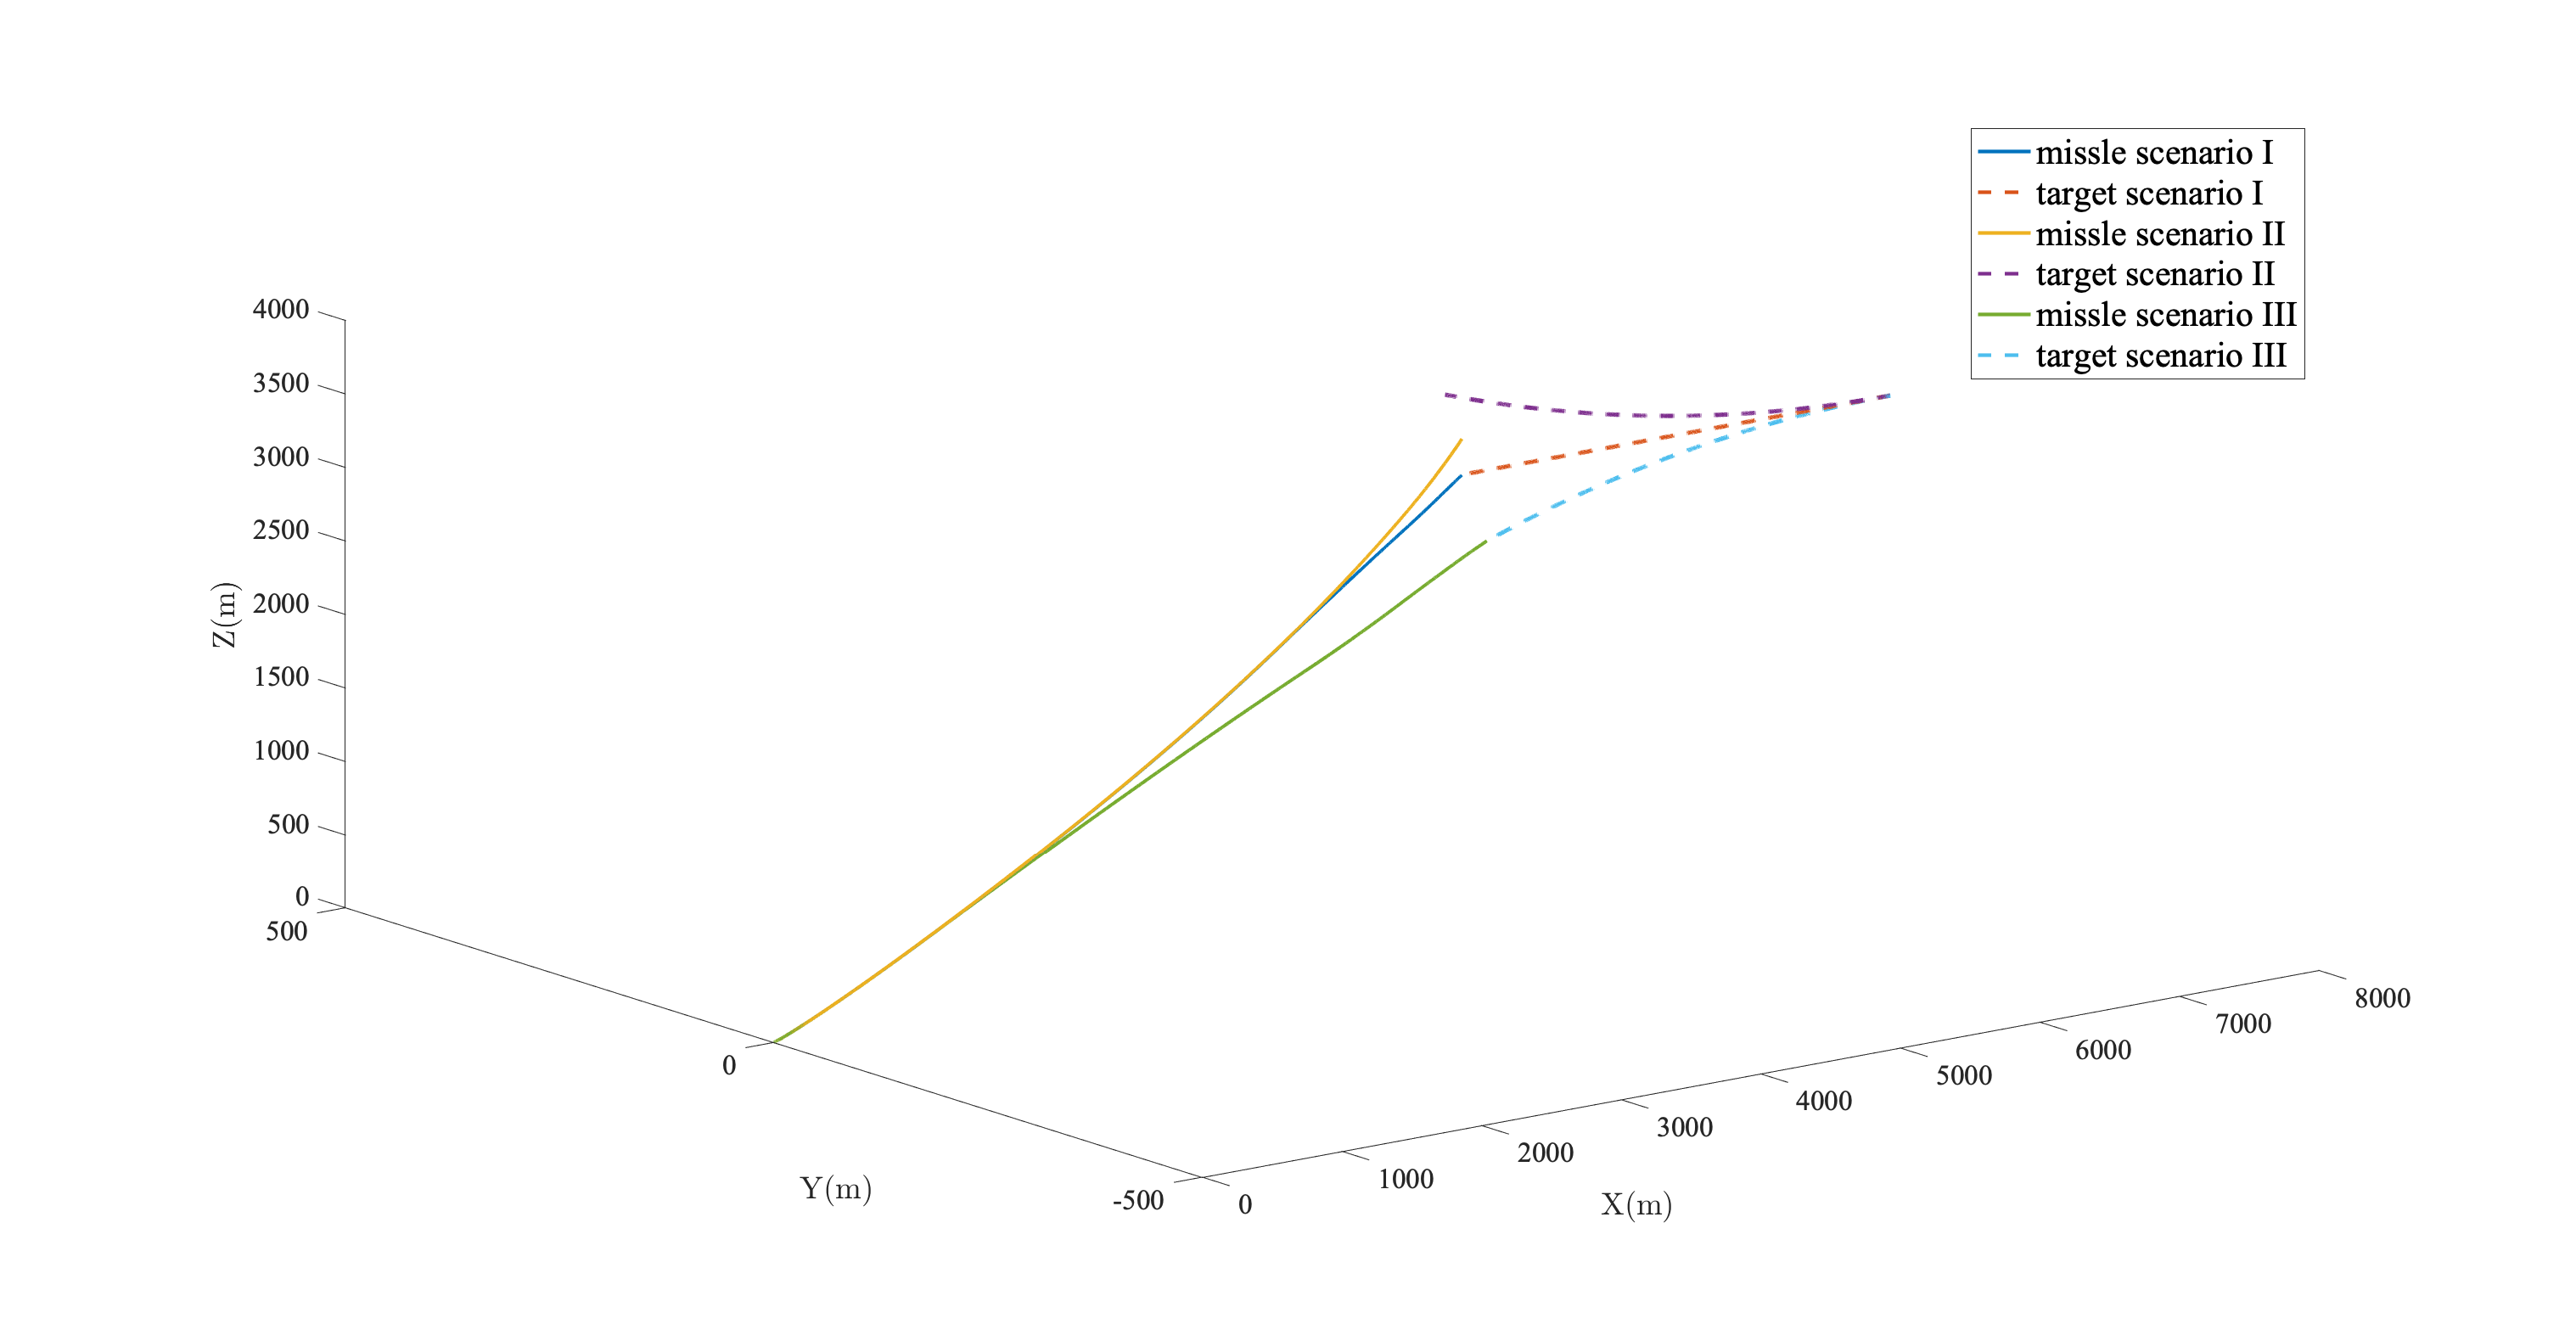
\includegraphics[width=\linewidth]{../Figure/m/3DoF_missle_vs_target_state_lead_angle1_all_in}
	\caption{مقایسه موقعیت موشک و هدف به صورت سه بعدی در یک نمودار در قانون هدایت فرمان به خط دید همراه با مانور هدف
	}
\end{figure}

\begin{figure}[H]
	\centering
	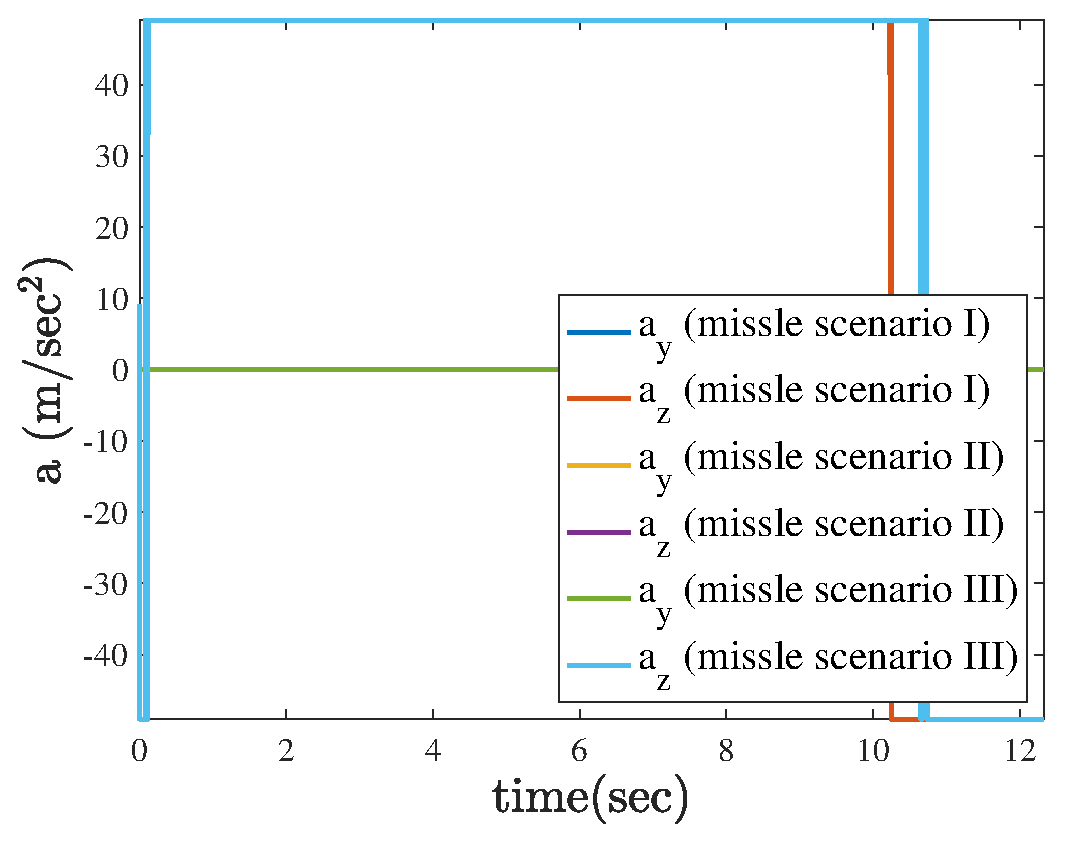
\includegraphics[width=.75\linewidth]{../Figure/m/command}
	\caption{مقایسه فرمان موشک در قانون هدایت فرمان به خط دید همراه با مانور هدف}
	
\end{figure}

\begin{figure}[H]
	\centering
	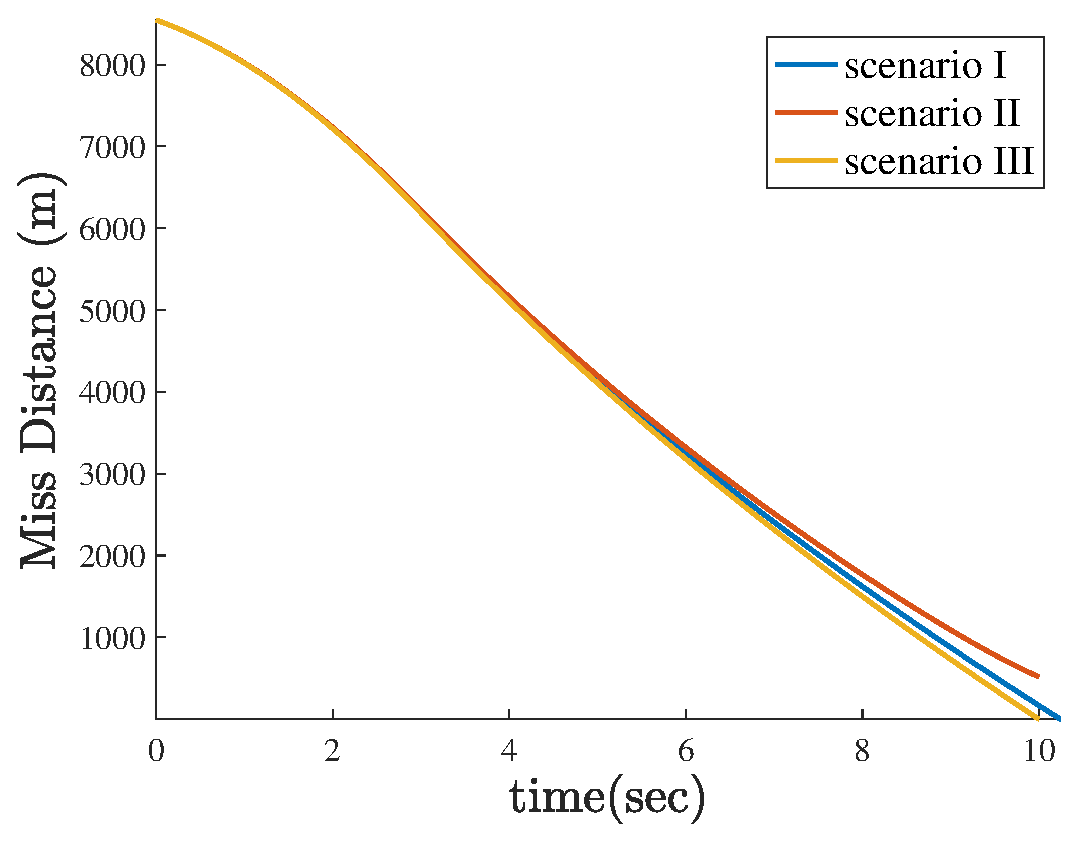
\includegraphics[width=.75\linewidth]{../Figure/m/miss_distance}
	\caption{مقایسه فاصله ازدست‌دهی موشک در قانون هدایت فرمان به خط دید همراه با مانور هدف}
\end{figure}


\begin{table}[H]
	\caption{فاصله ازدست‌دهی در قانون هدایت فرمان به خط دید همراه با مانور هدف}
	\centering
	\begin{tabular}{cc}
		\hline
		\lr{Miss Distance (m)} & \lr{Scenario} \\
		\hline
		\lr{2.1472}  &\lr{I}   \\
		\lr{343.6202 }&\lr{II}   \\
		\lr{0.6308}&\lr{II}   \\
		\hline
	\end{tabular}
\end{table}

